%\documentclass{article}
%\usepackage[utf8]{inputenc}

%\title{CUFCTLDLBD End of Semester Template}
%\author{Eddie Weill}
%\date{April 2017}

%\begin{document}

%\maketitle

%\section{Introduction}

%\end{document}


\documentclass[paper=a4, fontsize=11pt,twoside]{scrartcl} 

\usepackage[a4paper,pdftex]{geometry}	% A4paper margins
\setlength{\oddsidemargin}{5mm}			% Remove 'twosided' indentation
\setlength{\evensidemargin}{5mm}

\usepackage[english]{babel}
\usepackage[protrusion=true,expansion=true]{microtype}	
\usepackage{amsmath,amsfonts,amsthm,amssymb}
\usepackage{graphicx}

% --------------------------------------------------------------------
% Definitions (do not change this)
% --------------------------------------------------------------------
\newcommand{\HRule}[1]{\rule{\linewidth}{#1}} 	% Horizontal rule

\makeatletter							% Title
\def\printtitle{%						
	{\centering \@title\par}}
\makeatother									

\makeatletter							% Author
\def\printauthor{%					
	{\centering \large \@author}}				
\makeatother					

% --------------------------------------------------------------------
% Metadata (Change this)
% --------------------------------------------------------------------
\title{	\normalsize \textsc{Creative Inquiry: Deep Learning/Big Data} 	% Subtitle
	\\[2.0cm]								% 2cm spacing
	\HRule{0.5pt} \\						% Upper rule
	\LARGE \textbf{\uppercase{DLBD End-of-Semester Report}}	% Title
	\HRule{2pt} \\ [0.5cm]		% Lower rule + 0.5cm spacing
	\normalsize \today			% Todays date
}

\author{
	Your Name\\	
	Clemson University\\	
	Department of Electrical and Computer Engineering\\
	\texttt{your@email.com} \\
}


\begin{document}
% ------------------------------------------------------------------------------
% Maketitle
% ------------------------------------------------------------------------------
\thispagestyle{empty}		% Remove page numbering on this page

\printtitle					% Print the title data as defined above
\vfill
\printauthor				% Print the author data as defined above
\newpage


% ------------------------------------------------------------------------------
% Begin document
% ------------------------------------------------------------------------------

\setcounter{page}{1}		% Set page numbering to begin on this page
\section{Introduction}

In this section you will describe your experience in the CI.  Good topics to discuss include your exposure to topics otherwise inaccessible to undergraduate students, or any relevant topics or interest that you feel you would like to research or pursue in the future because of your participation in the CI. If this CI has had any impact on your understanding or interest in pursuing a graduate degree, feel free to mention this as well.

\section{Technical Knowledge Gained}

In this section you can elaborate on any kind of knowledge gained during the course of this semester.  This could be anything from creation of a large dataset to understanding deep learning techniques to training networks to recognize certain objects.  Be as elaborate as you feel necessary, but make sure to convey all the knowledge that you have gained throughout the semester while participating in this CI.

\section{Results}

In this section you will put any relevant results that you have achieved during the semester.  You should focus on results that show the dataset you have created as well as the training that you were able to accomplish.  Make sure to fully explain all the images or tables provided.  For example, if you have an image with a 3 labels and your network only detects 2 of them, try and make some justification of why you feel the last label was not detected.  If you are able to get performance metrics (precision, recall, mAP, etc.) for your network as well, make sure to put those in this section in either a table format or some way that it is easily distinguishable.

\subsection{Single Class Detection}
\subsection{20-Class Detection}
\subsection{Final Project}

\section{Conclusions and Future Work}

In this section you can make conclusions about the results that you achieved during the course of the semester.  If you have any ideas for continued work in the CI, you can put those in this section as well.  For example, if there is a particular project which you think will fit well in the CI and you want to work on it, this would be a good place to explain it briefly.

\section*{TeX Helpful Hints}\label{design}

Below you will find a few helpful hints for creating different objects (i.e. tables, mathmatics, etc.) in a tex document.  This will be removed from your document before turning in.

\subsection*{Text}

Use \texttt{section}s and \texttt{subsection}s to organize your document. \LaTeX{} handles all the formatting and numbering automatically. Use \texttt{ref} and \texttt{label} for cross-references --- this is Section~\ref{design}, for example.
You can also add math formula in sentences such as $\frac{\pi}{2}$.
\subsection*{Tables and Figures}
You can create a table as shown in \ref{tab:table1}.  You can also go to the following URL (or do a simple Google search for Latex tables): https://www.sharelatex.com/learn/Tables.
\begin{table}
	\centering
	\caption{Caption for the table.}
	\label{tab:table1}
	\begin{tabular}{l|c||r}
		\hline
		1 & 2 & 3\\
		\hline
		a & b & c\\
		\hline
	\end{tabular}
\end{table}

You can upload your figures (JPEG, PNG, or PDF) and inlude them in the document as shown in \ref{fig:your-figure}.

% Commands to include a figure:
% NOTE: the [h!] will put a figure exactly in LaTeX and without it, will go at the top of page
\begin{figure}[h!]
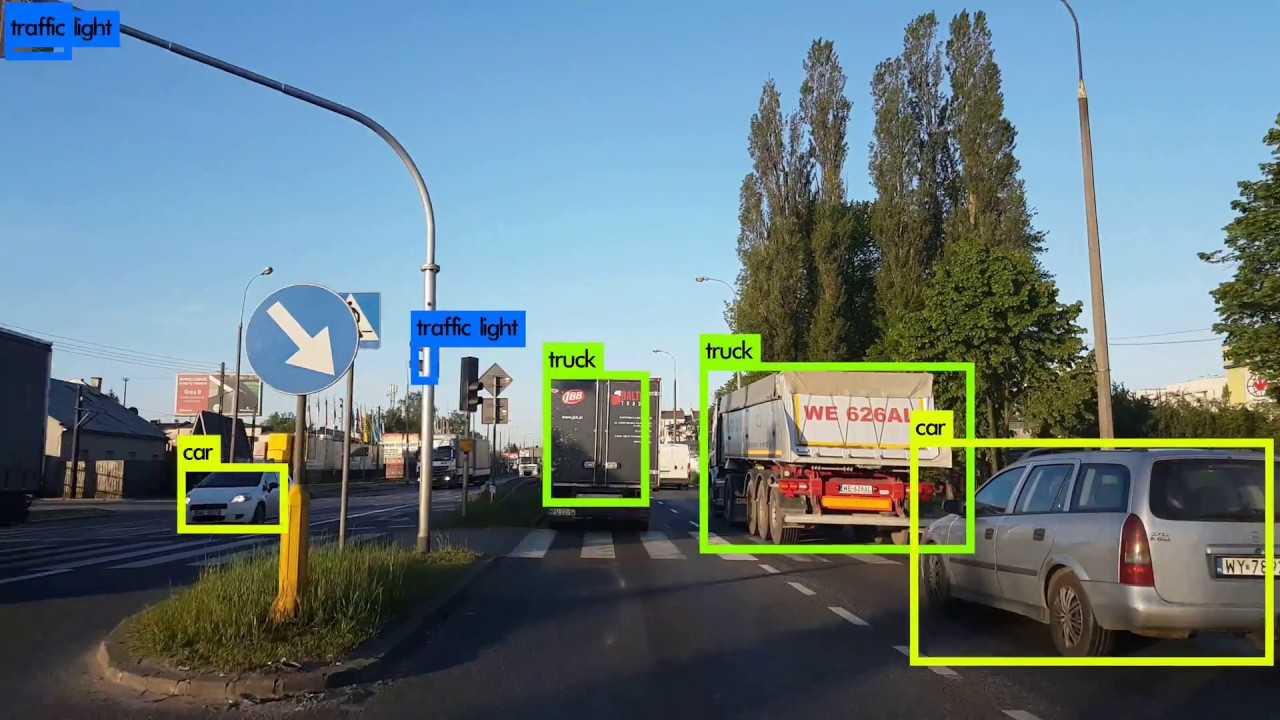
\includegraphics[width=\textwidth]{detection.jpg}
\caption{\label{fig:your-figure}Example Label File}
\end{figure}

\subsection*{Mathematics}

\LaTeX{} is great at typesetting mathematics. Let $X_1, X_2, \ldots, X_n$ be a sequence of independent and identically distributed random variables with $\text{E}[X_i] = \mu$ and $\text{Var}[X_i] = \sigma^2 < \infty$, and let
$$S_n = \frac{X_1 + X_2 + \cdots + X_n}{n}
= \frac{1}{n}\sum_{i}^{n} X_i$$
denote their mean. Then as $n$ approaches infinity, the random variables $\sqrt{n}(S_n - \mu)$ converge in distribution to a normal $\mathcal{N}(0, \sigma^2)$.

\subsection*{Lists}

You can make lists with automatic numbering \dots

\begin{enumerate}
	\item Like this,
	\item and like this.
\end{enumerate}
\dots or bullet points \dots
\begin{itemize}
	\item Like this,
	\item and like this.
\end{itemize}

\end{document}